\documentclass[11pt,a4paper]{article}

\usepackage[margin=1in]{geometry}
\usepackage{graphicx}
\usepackage{booktabs}
\usepackage{tabularx}
\usepackage{array}
\usepackage{multirow}
\usepackage{amsmath,amssymb}
\usepackage{float}
\usepackage{placeins}
\usepackage{xcolor}
\usepackage{url}
\usepackage{hyperref}
\usepackage[numbers,sort&compress]{natbib}

\graphicspath{{figures/}}
\hypersetup{
  colorlinks=true,
  linkcolor=blue!50!black,
  citecolor=blue!50!black,
  urlcolor=blue!50!black
}

\newcommand{\rocauc}{AUC-ROC}
\newcommand{\prauc}{AUC-PR}
\newcommand{\far}{FAR}
\newcommand{\miss}{Miss}
\newcommand{\hi}{HI}

\title{A Calibration-Aware Fuzzy Health Index for Normal-Only Bearing Anomaly Detection: Strict Generalization Validation and External Paderborn Evaluation}

\author{
Anonymous Author(s)\\
Department of Artificial Intelligence Application Engineering\\
Anonymous Institution\\
\texttt{anonymous@example.com}
}

\date{}

\begin{document}
\maketitle

\begin{abstract}
Public bearing benchmarks have enabled rapid progress in data-driven condition monitoring, yet many reported results remain difficult to translate into deployable anomaly detection systems. A common reason is that experiments are often evaluated under window-level random splits, balanced fault distributions, and model-centric metrics such as \rocauc. These settings can overstate practical performance when sliding windows from the same file, operating load, or bearing condition appear in both training and testing. This paper presents a reproducible normal-only bearing anomaly detection workflow that treats threshold calibration and health-state interpretation as first-class components rather than post-processing details. The proposed pipeline trains only on normal vibration windows, evaluates VAE, CNN-AE, LSTM-AE and Isolation Forest models under strict CWRU protocols, extends validation to the Paderborn bearing dataset, and converts calibrated anomaly scores into a fuzzy health index with normal, warning, fault and uncertain regions. On CWRU, neural reconstruction models retain high ranking performance under load-wise, fault-size-wise and file-wise splits, but false alarm behavior depends strongly on the threshold policy. On Paderborn, the same framework exposes a more realistic external-domain challenge: ranking quality remains informative, whereas thresholded decisions become substantially harder, especially when conservative percentile or robust MAD thresholds are used. These results show that deployment-oriented bearing anomaly detection should report not only ranking metrics, but also calibration transfer, false alarm rate, miss rate, uncertainty rate, inference latency and model footprint. The main contribution is therefore not another high-accuracy CWRU classifier, but a calibration-aware, reproducible and interpretable workflow for normal-only industrial health monitoring research.
\end{abstract}

\noindent\textbf{Keywords:} bearing anomaly detection; normal-only training; threshold calibration; fuzzy health index; variational autoencoder; Paderborn bearing dataset; CWRU; reproducible condition monitoring.

\section{Introduction}

Rotating machinery is central to manufacturing, transportation, energy systems and many other industrial environments. Rolling bearings are among the components most frequently monitored because local faults can propagate quickly from small surface defects to severe equipment downtime. For this reason, vibration-based bearing diagnosis has become one of the most active areas in condition monitoring and predictive maintenance \citep{randall2011tutorial,smith2015cwru}. Public datasets such as the Case Western Reserve University (CWRU) bearing data and the Paderborn bearing dataset have made this research easier to reproduce and compare \citep{cwru_dataset,lessmeier2016paderborn,paderborn_datacenter}.

The availability of benchmarks, however, has also created a methodological risk. Many bearing fault diagnosis studies are framed as supervised classification tasks with known fault types, balanced class distributions and random train-test splits. Such settings are useful for algorithm development, but they do not fully represent early-stage industrial monitoring. In real plants, fault examples are rare, fault labels are expensive, and machines may operate under loads, speeds, bearing units and environmental conditions that differ from the data used during model selection. In this setting, the more realistic problem is often normal-only anomaly detection: a model is trained on healthy behavior and must raise alarms when the observed signal no longer resembles the learned normal state.

Normal-only anomaly detection changes the scientific question. The question is no longer only whether a model can rank normal and faulty windows correctly under a benchmark split. A deployable system must also decide where to place the alarm threshold, how the threshold behaves under load or dataset shift, how often false alarms occur, how often faults are missed, and how an operator should interpret borderline scores. These questions are especially important when a benchmark is highly separable. For example, CWRU experiments can produce nearly perfect \rocauc\ values for multiple model families, making it difficult to argue that a particular neural architecture is practically superior. Under such conditions, threshold calibration and generalization protocols become more informative than another marginal change in reconstruction architecture.

This paper responds to that gap by repositioning the study around calibration-aware anomaly detection. Instead of presenting a VAE pipeline only as a model-performance result, we develop a reproducible workflow that evaluates the complete path from data preparation to health-state decision. The workflow begins with normal-only training, applies strict generalization protocols to reduce sliding-window leakage, evaluates both neural and classical anomaly models, studies dataset-specific threshold policies, and maps calibrated anomaly scores into a fuzzy health index. The fuzzy layer is not intended to replace the anomaly score. Rather, it provides a structured way to express normal, warning, fault and uncertain regions, which is more aligned with industrial decision support than a single binary threshold.

Before introducing the technical details, it is useful to state what this work deliberately does not claim. We do not claim a new state-of-the-art bearing classifier. We also do not claim that CWRU alone is sufficient evidence of industrial generalization. The objective is more modest and, we argue, more useful: to show how the evaluation of normal-only bearing anomaly detection changes when strict splits, external validation, threshold calibration and fuzzy health interpretation are considered together.

The contributions of this paper are summarized as follows:
\begin{itemize}
  \item We present a reproducible normal-only bearing anomaly detection workflow that supports VAE, CNN-AE, LSTM-AE and Isolation Forest models under a common scoring and reporting interface.
  \item We evaluate the workflow using strict CWRU protocols, including load-wise, fault-size-wise and file-wise splits, to reduce the risk of optimistic sliding-window leakage.
  \item We extend the analysis to the Paderborn dataset using condition-wise, bearing-wise and file-wise protocols, showing that external bearing data create a substantially harder calibration problem than CWRU.
  \item We compare threshold calibration policies, including train-normal percentiles, validation-normal percentiles and robust MAD thresholds, and report their effects on \far, miss rate and F1.
  \item We integrate a fuzzy health index on top of calibrated anomaly scores, enabling interpretable normal, warning, fault and uncertain decisions while preserving model-agnostic score inputs.
  \item We report deployment-relevant evidence, including CPU inference latency, model size and a reproducibility checklist.
\end{itemize}

The remainder of the paper is organized as follows. Section~\ref{sec:related_work} reviews related work and clarifies the methodological position of this study. Section~\ref{sec:methods} defines the normal-only anomaly detection problem and presents the proposed workflow. Section~\ref{sec:experimental_design} describes datasets, protocols, models and metrics. Section~\ref{sec:results} reports the experimental results. Section~\ref{sec:discussion} discusses the implications for industrial deployment and journal-level research positioning. Section~\ref{sec:conclusion} concludes the paper.

\section{Related Work}
\label{sec:related_work}

The present work connects several research streams that are often studied separately: bearing fault diagnosis, unsupervised anomaly detection, domain generalization, threshold calibration and fuzzy health assessment. This section therefore does not review every deep learning architecture proposed for bearing diagnosis. Instead, it focuses on the evaluation assumptions that determine whether a method can support normal-only industrial monitoring.

\subsection{Bearing fault diagnosis benchmarks}

CWRU is one of the most widely used public datasets for rolling bearing diagnostics. It provides normal and faulty vibration signals collected under controlled motor-load conditions, and has been repeatedly used to test signal processing and machine learning methods \citep{cwru_dataset,smith2015cwru}. Smith and Randall \citep{smith2015cwru} emphasized that the dataset is valuable but should be used carefully because benchmark structure, fault characteristics and evaluation protocol strongly influence conclusions. This warning remains relevant in modern deep learning studies: if highly overlapping windows from the same experimental file appear in both training and testing, performance can reflect local similarity rather than true generalization.

The Paderborn bearing dataset provides a broader external benchmark. It includes healthy bearings, artificially damaged bearings and real damages produced through accelerated lifetime tests, with measurements obtained under different operating conditions \citep{lessmeier2016paderborn,paderborn_datacenter}. Compared with CWRU, Paderborn is more useful for testing whether a workflow remains meaningful when bearing identities, damage types and operating conditions vary. This makes it a natural external dataset for evaluating whether a normal-only anomaly detection pipeline is robust beyond a clean benchmark.

\subsection{Deep learning for bearing diagnosis}

Deep learning has become dominant in bearing fault diagnosis because convolutional, recurrent and attention-based models can learn features directly from raw vibration signals. CNN-based methods are effective for local temporal patterns and time-frequency representations, while LSTM-based models are often used when sequence dependency is emphasized. Transformer and self-supervised variants have recently been explored to reduce dependence on manually designed features and improve representation transfer \citep{li2024cnnreview,masked2025swin,phm2024selfsupervised}. These developments are valuable, but many of them remain tied to classification protocols with labeled fault categories.

Reconstruction-based anomaly detection provides a different route. Autoencoders, variational autoencoders and related models can be trained on normal data and then use reconstruction error, latent likelihood proxies or hybrid scores to identify abnormal behavior \citep{kingma2014vae,zhao2023hybrid}. This is closer to industrial deployment when only healthy data are available. However, the reconstruction score alone is not a decision rule. A threshold must be selected, and the threshold must remain stable enough across operating conditions to support alarms. In practice, this calibration step often receives less attention than the architecture.

\subsection{Domain shift and strict generalization}

Condition monitoring systems frequently face domain shift. Loads, speeds, sensors, bearing units, lubrication conditions and installation differences can alter the distribution of vibration signals. Domain adaptation methods address this issue by aligning source and target representations, often using adversarial training, subdomain adaptation or distribution discrepancy losses \citep{dada2021bearing,luo2022dsan,iseanet2024bearing}. Open-set and source-free adaptation methods further consider unknown or unavailable fault domains \citep{sourcefree2025bearing}. These approaches are important, but they may assume access to target-domain data or fault labels that are not always available during deployment.

Our study uses a simpler but stricter evaluation perspective. Instead of adapting to the target condition, we hold out loads, fault sizes, files, operating conditions or bearing groups and measure how the entire anomaly detection workflow behaves. This does not solve domain shift by itself. Rather, it makes the shift visible and prevents a model from appearing stronger because of accidental overlap between training and test windows.

\subsection{Threshold calibration and deployment metrics}

\rocauc\ is a ranking metric. It measures whether abnormal examples tend to receive higher anomaly scores than normal examples, but it does not specify an alarm threshold. In highly imbalanced industrial environments, \prauc, false alarm rate, miss rate and threshold sensitivity can be more directly relevant. A model with excellent ranking ability may still be unacceptable if a practical threshold generates too many false alarms under a new load. Conversely, a conservative threshold may lower false alarms while missing most faults.

Threshold calibration is therefore not merely a post-processing detail. Percentile thresholds estimated from training-normal scores, validation-normal scores or robust statistics such as median absolute deviation encode different risk preferences. They also respond differently to dataset shift. This paper evaluates these threshold policies explicitly and argues that calibration transfer should be reported alongside model ranking.

\subsection{Fuzzy health assessment}

Fuzzy logic has a long history in control and health assessment because it supports graded decisions instead of hard class boundaries \citep{zadeh1965fuzzy}. In condition monitoring, fuzzy rules are often used to combine indicators into interpretable health states. This is appealing for industrial users: an operator may benefit from knowing whether a score belongs to a warning region or an uncertain region, not only whether it crosses one alarm line.

In this work, fuzzy logic is used as a model-agnostic decision layer. The inputs are normalized anomaly scores produced by VAE, CNN-AE, LSTM-AE or Isolation Forest models. The outputs are health index values and decision regions. The purpose is to improve interpretability and make threshold uncertainty explicit, especially under external validation where a single binary cutoff can hide important ambiguity.


\begin{table*}[t]
\centering
\caption{Positioning of the present work relative to recent bearing fault diagnosis studies.}
\label{tab:literature_positioning}
\small
\setlength{\tabcolsep}{5pt}
\renewcommand{\arraystretch}{1.18}
\begin{tabularx}{\textwidth}{>{\raggedright\arraybackslash}p{3.2cm}
>{\raggedright\arraybackslash}X
>{\raggedright\arraybackslash}X}
\toprule
Study direction & Common emphasis and limitation & Position of this study \\
\midrule
Deep supervised diagnosis and CNN/Transformer models & Emphasizes high classification accuracy under known fault classes, but usually requires labeled faults and can rely on condition-overlapping splits. & Studies normal-only anomaly detection and reports strict generalization protocols. \\
Autoencoder and VAE novelty detection & Uses reconstruction error as an anomaly score, while threshold choice and alarm behavior are often treated as secondary details. & Treats calibration and health decision rules as primary workflow components. \\
Self-supervised bearing representation learning & Learns transferable features from unlabeled signals, but is often evaluated as downstream classification. & Keeps the deployment task as abnormality screening without fault labels in training. \\
Domain adaptation and open-set diagnosis & Targets load, speed and dataset shift, but may assume target-domain adaptation data or source labels. & Compares holdout protocols and calibration behavior across CWRU and Paderborn. \\
Fuzzy health assessment & Provides interpretable condition categories, but is often separated from modern anomaly scores. & Connects fuzzy membership functions to calibrated anomaly scores. \\
\bottomrule
\end{tabularx}
\end{table*}


\section{Methods}
\label{sec:methods}

This section introduces the proposed workflow in the order an industrial monitoring system would use it: define the normal-only task, build windows from vibration signals, train anomaly models, calibrate thresholds and convert scores into fuzzy health decisions. To avoid the abrupt structure that often appears in project reports, each subsection is connected to the practical question it answers.

\subsection{Problem definition}

The first question is what information is allowed during training. We consider a normal-only setting. Let $x \in \mathbb{R}^{L}$ denote a vibration window of length $L$. During training, the model observes only windows sampled from normal bearing operation:
\begin{equation}
\mathcal{D}_{train}=\{x_i^{(n)}\}_{i=1}^{N}.
\end{equation}
Fault labels are not used to learn the model or tune the anomaly representation. Fault windows appear only in held-out evaluation sets. This setting reflects practical plants where normal data are plentiful but labeled faults are rare, costly or unavailable.

An anomaly model produces a continuous score
\begin{equation}
s(x)=g_{\theta}(x),
\end{equation}
where larger values indicate stronger deviation from learned normal behavior. For reconstruction models, $s(x)$ is based on reconstruction error. For Isolation Forest, $s(x)$ is the transformed isolation score. A binary alarm is then obtained by comparing the score with a threshold $\tau$:
\begin{equation}
\hat{y}(x)=\mathbb{I}[s(x)>\tau].
\end{equation}
This separation between score generation and threshold selection is important. A model may rank faults well but still fail to provide a stable threshold across loads or datasets.

\subsection{Workflow overview}

After defining the task, the next question is how the full pipeline is organized. Figure~\ref{fig:pipeline} shows the redesigned workflow. The pipeline begins with public bearing datasets and normal-only training windows. Strict protocols then define which loads, fault sizes, files, operating conditions or bearing groups are withheld. Anomaly models are trained under the same input-output interface, and their scores are passed to calibration policies. Finally, calibrated scores are converted into fuzzy health states and summarized using deployment-oriented metrics.

\begin{figure*}[t]
  \centering
  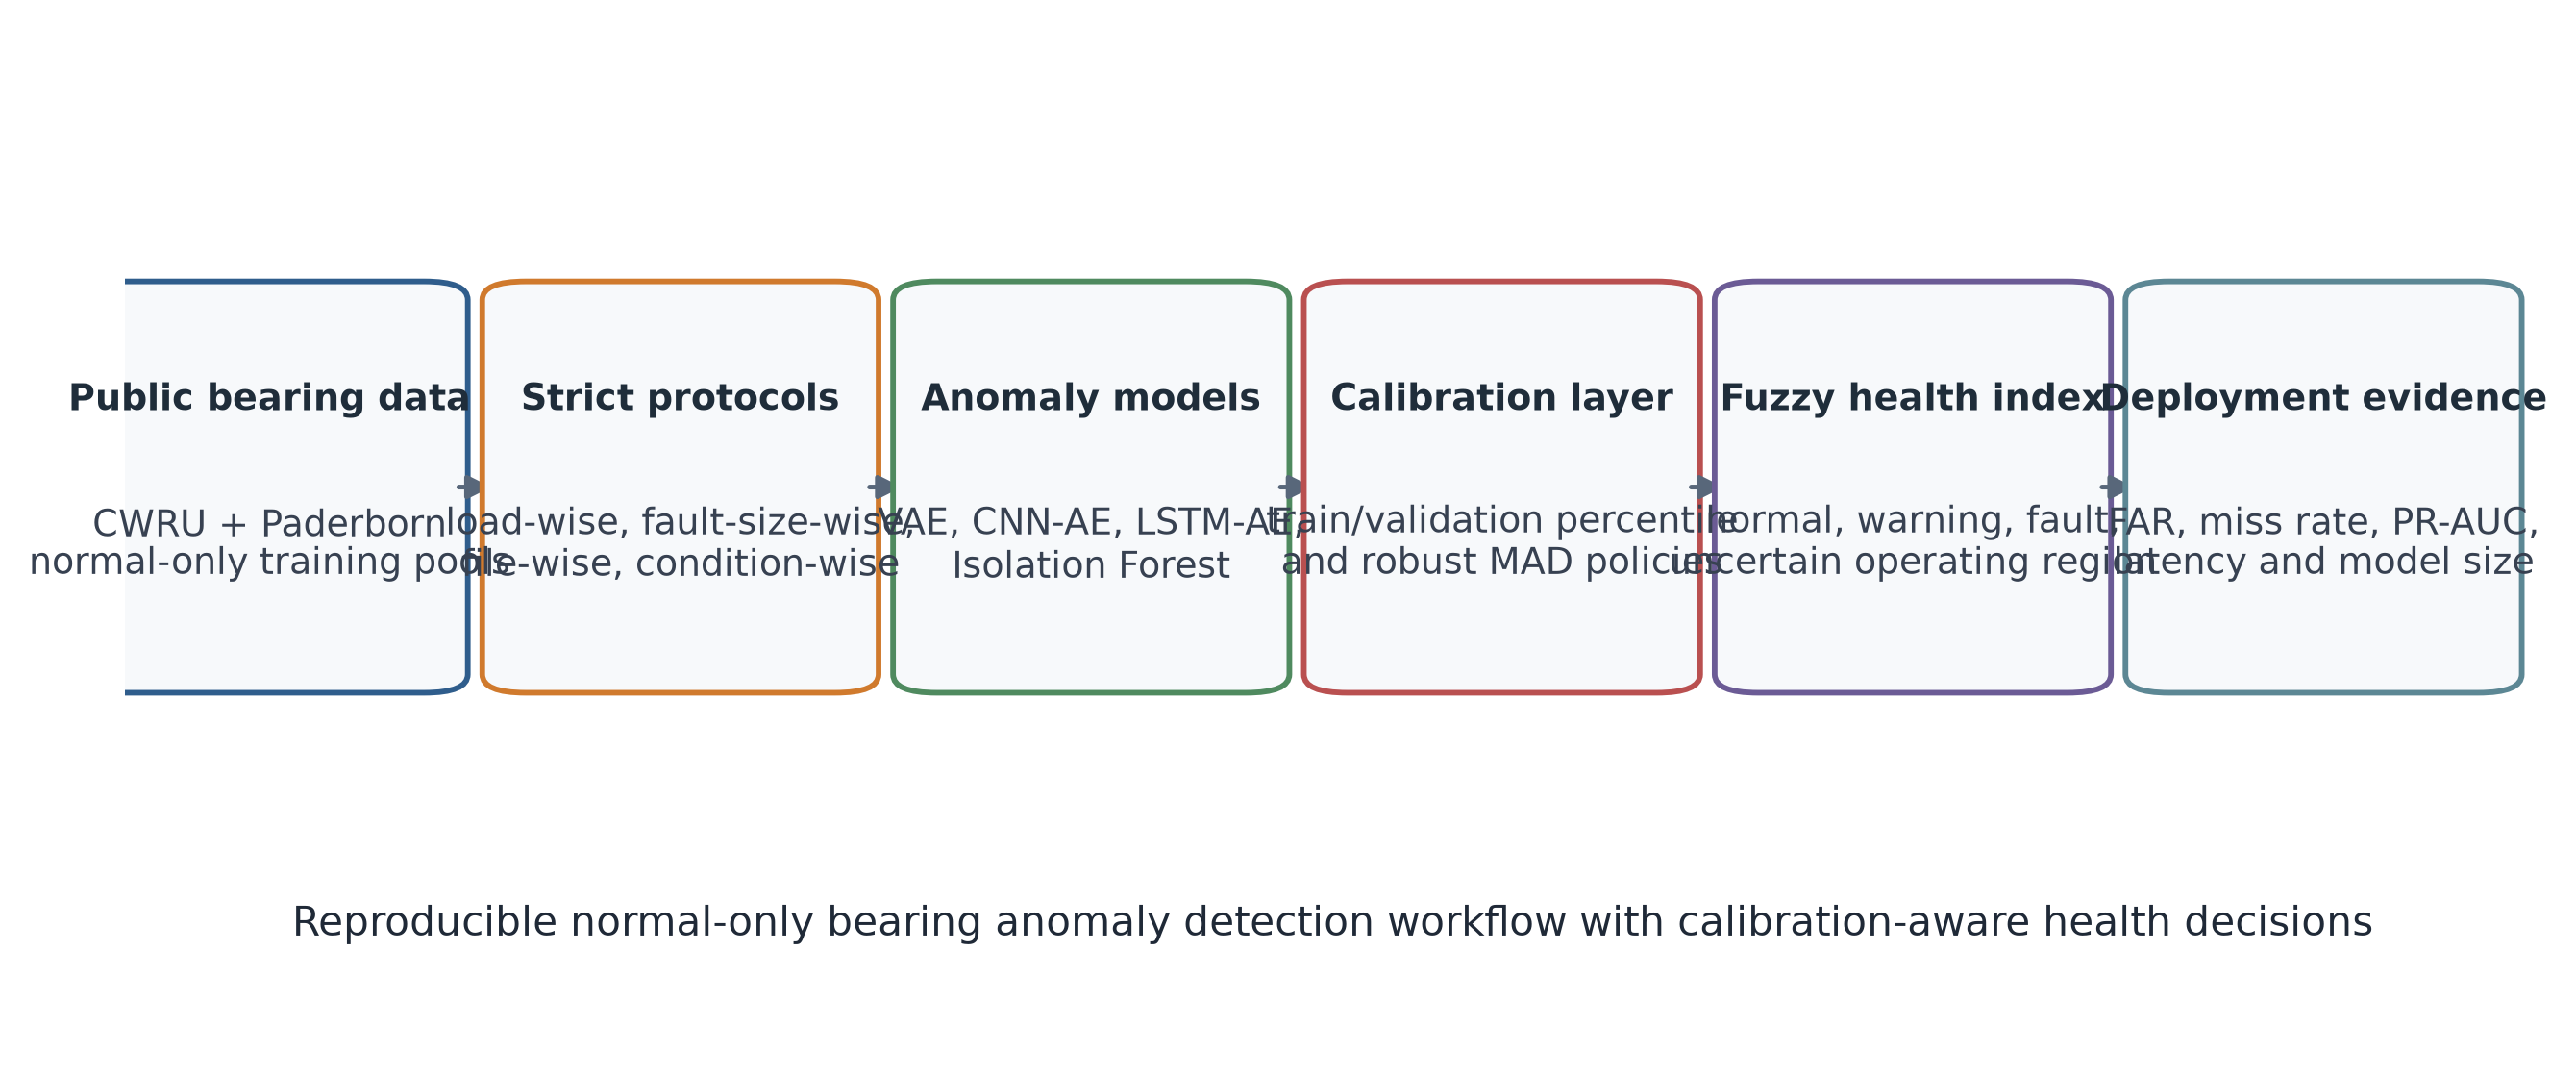
\includegraphics[width=\textwidth]{fig01_research_pipeline.png}
  \caption{Proposed calibration-aware normal-only bearing anomaly detection workflow. The redesigned pipeline emphasizes strict generalization protocols, threshold calibration and fuzzy health-state interpretation rather than only model accuracy.}
  \label{fig:pipeline}
\end{figure*}

The workflow is intentionally modular. A new anomaly model can be added if it produces a scalar score. A new dataset can be added if normal windows and held-out evaluation groups are defined. A new threshold policy can be compared without retraining the anomaly model. This modularity is central to the reproducibility goal of the paper.

\subsection{Windowing and normalization}

The workflow operates on fixed-length vibration windows. Given a raw signal $r(t)$, windows are extracted using length $L$ and stride $S$. CWRU experiments use $L=1024$ and $S=512$ to maintain continuity with the original conference version and common benchmark practice. Paderborn experiments use $L=8192$ as the main external validation setting because preliminary sensitivity analysis showed that longer windows provide more stable information under its broader operating conditions. Shorter Paderborn windows are retained as a sensitivity analysis rather than the primary claim.

Each window is standardized using statistics estimated from the corresponding training-normal data. This prevents test information from entering preprocessing. When classical baselines use statistical features, the feature normalization is also estimated from training-normal data only.

\subsection{Anomaly models}

The next question is whether the workflow depends on a single architecture. To avoid this limitation, four model families are evaluated.

\textbf{Variational autoencoder.} The VAE learns a latent distribution for normal vibration windows. The encoder estimates latent parameters, the decoder reconstructs the input, and the training objective combines reconstruction loss with a KL regularization term \citep{kingma2014vae}. The anomaly score is the reconstruction error. In this paper, the VAE is treated as a representative probabilistic reconstruction model, not as a guaranteed superior architecture.

\textbf{CNN autoencoder.} The CNN-AE uses convolutional encoding and decoding layers to reconstruct local vibration patterns. It is included because convolutional models are strong baselines for one-dimensional bearing signals and often capture impulse-like fault signatures efficiently.

\textbf{LSTM autoencoder.} The LSTM-AE reconstructs the window through recurrent sequence modeling \citep{hochreiter1997lstm}. It is included to test whether temporal sequence modeling changes generalization behavior relative to convolutional reconstruction.

\textbf{Isolation Forest.} Isolation Forest is a classical anomaly detection method based on the idea that anomalies are easier to isolate using random partitions \citep{liu2008iforest}. It is used with statistical vibration features and serves as a lightweight non-neural baseline. It is also useful for studying threshold policies because it has low computational cost and stable scalar scores.

\subsection{Threshold calibration}

Once anomaly scores are available, the most important deployment question becomes threshold selection. We evaluate five policies:
\begin{align}
\tau_{train95} &= Q_{0.95}(s(\mathcal{D}_{train}^{normal})),\\
\tau_{train99} &= Q_{0.99}(s(\mathcal{D}_{train}^{normal})),\\
\tau_{val95} &= Q_{0.95}(s(\mathcal{D}_{val}^{normal})),\\
\tau_{val99} &= Q_{0.99}(s(\mathcal{D}_{val}^{normal})),\\
\tau_{mad5} &= \mathrm{median}(s) + 5 \cdot \mathrm{MAD}(s).
\end{align}
The percentile policies represent practical choices when normal validation data are available. The robust MAD policy represents a conservative robust-statistics alternative. These thresholds are not optimized on fault labels. Their purpose is to test how normal-only calibration behaves when the test condition changes.

\subsection{Fuzzy health index}

A hard threshold divides all windows into normal and abnormal states, but industrial monitoring often requires a softer interpretation. We therefore define a fuzzy health index $h(x)\in[0,1]$ using calibrated anomaly scores. Low normalized scores have high membership in the normal region, intermediate scores have warning or uncertain membership, and high scores have high membership in the fault region. The decision layer supports two operating policies: warning-as-alarm and fault-only alarm. The former is more sensitive, while the latter is more conservative.

The fuzzy layer has two roles. First, it provides an interpretable health index that can be trended over time. Second, it makes ambiguity visible through the uncertain rate. This is particularly important for Paderborn, where external-domain variation creates score overlap that would be hidden by a single binary threshold.

\section{Experimental Design}
\label{sec:experimental_design}

The method is evaluated through a sequence of increasingly strict experiments. The design starts with CWRU because it is controlled and widely recognized, then moves to Paderborn because it better tests external validity. This section describes the datasets, protocols, metrics and reproducibility artifacts used to support the claims.

\subsection{Datasets and protocols}

Table~\ref{tab:dataset_protocols} summarizes the datasets and protocol roles. CWRU is used to test whether the original high benchmark performance survives stricter splitting. Three protocols are used: load-wise, fault-size-wise and file-wise. Load-wise split holds out a motor load. Fault-size-wise split holds out a fault diameter. File-wise split holds out source files so overlapping windows from the same file cannot appear on both sides of the evaluation boundary.

Paderborn is used as an external validation dataset. Three protocols are retained: condition-wise, bearing-wise and file-wise. Condition-wise split holds out operating conditions. Bearing-wise split holds out bearing identities or damage groups. File-wise split again reduces leakage from overlapping windows. These protocols correspond to different industrial questions: transfer across operation, transfer across bearing state and avoidance of window-level leakage.

\begin{table}[t]
\centering
\caption{Datasets and strict generalization protocols used in the study.}
\label{tab:dataset_protocols}
\small
\begin{tabular}{lllll}
\toprule
Dataset & Signal source & Training assumption & Strict protocols & Main role \\
\midrule
CWRU & Drive-end vibration & Normal windows only & load-wise, fault-size-wise, file-wise & Controlled benchmark for protocol stress testing \\
Paderborn & Vibration data from multiple bearings and conditions & Normal windows only & condition-wise, bearing-wise, file-wise & External validation under stronger operating and bearing variation \\
\bottomrule
\end{tabular}
\end{table}

\subsection{Metrics}

We report both ranking and thresholded metrics. Ranking metrics include \rocauc\ and \prauc. Thresholded metrics include precision, recall, F1, false alarm rate and miss rate:
\begin{equation}
\mathrm{FAR}=\frac{FP}{FP+TN}, \qquad
\mathrm{Miss}=\frac{FN}{FN+TP}.
\end{equation}
For fuzzy decisions, we also report uncertain rate and mean health index for normal and fault windows. For deployment evidence, we report CPU inference time per window, model size and parameter count.

This metric set is intentionally broader than \rocauc. In industrial monitoring, an operator experiences alarms and misses, not only ranking curves. A good research pipeline should therefore reveal when a model ranks well but calibrates poorly.

\subsection{Reproducibility}

All experiments are designed to produce CSV outputs, figure files and LaTeX tables. The released workflow records split definitions, threshold strategies, model names, score metrics, confusion-matrix counts and efficiency statistics. Table~\ref{tab:reproducibility} lists the main reproducibility elements.

\begin{table}[t]
\centering
\caption{Reproducibility checklist for the released experimental pipeline.}
\label{tab:reproducibility}
\small
\begin{tabular}{lll}
\toprule
Component & Released element & Purpose \\
\midrule
Data preparation & Dataset download/preprocessing scripts & Recreates windowed normal-only training and held-out test splits \\
Protocols & Explicit load-wise, fault-size-wise, file-wise, condition-wise and bearing-wise split definitions & Avoids accidental sliding-window leakage and evaluates domain shift \\
Models & VAE, CNN-AE, LSTM-AE and Isolation Forest implementations & Supports neural and classical baselines under common scoring outputs \\
Calibration & Percentile and MAD threshold policies & Separates ranking quality from deployable alarm behavior \\
Outputs & CSV metrics, figures and LaTeX tables & Makes numerical claims traceable to generated artifacts \\
\bottomrule
\end{tabular}
\end{table}

\section{Results}
\label{sec:results}

The results are organized around the paper's central claim: model ranking, threshold calibration and interpretable health decision must be evaluated together. We first report strict CWRU results, then Paderborn external validation, threshold tradeoffs, fuzzy health interpretation and efficiency.

\subsection{Strict CWRU validation}

CWRU remains highly separable even under strict protocols. Figure~\ref{fig:cwru_models} and Table~\ref{tab:cwru_strict} show that VAE, CNN-AE and LSTM-AE retain near-perfect ranking performance in many cases. However, the thresholded behavior is less uniform. Under validation-P99 calibration, false alarm rates for neural reconstruction models are higher in some file-wise and load-wise settings, while Isolation Forest gives lower false alarms at the cost of higher miss rates.

\begin{figure*}[t]
  \centering
  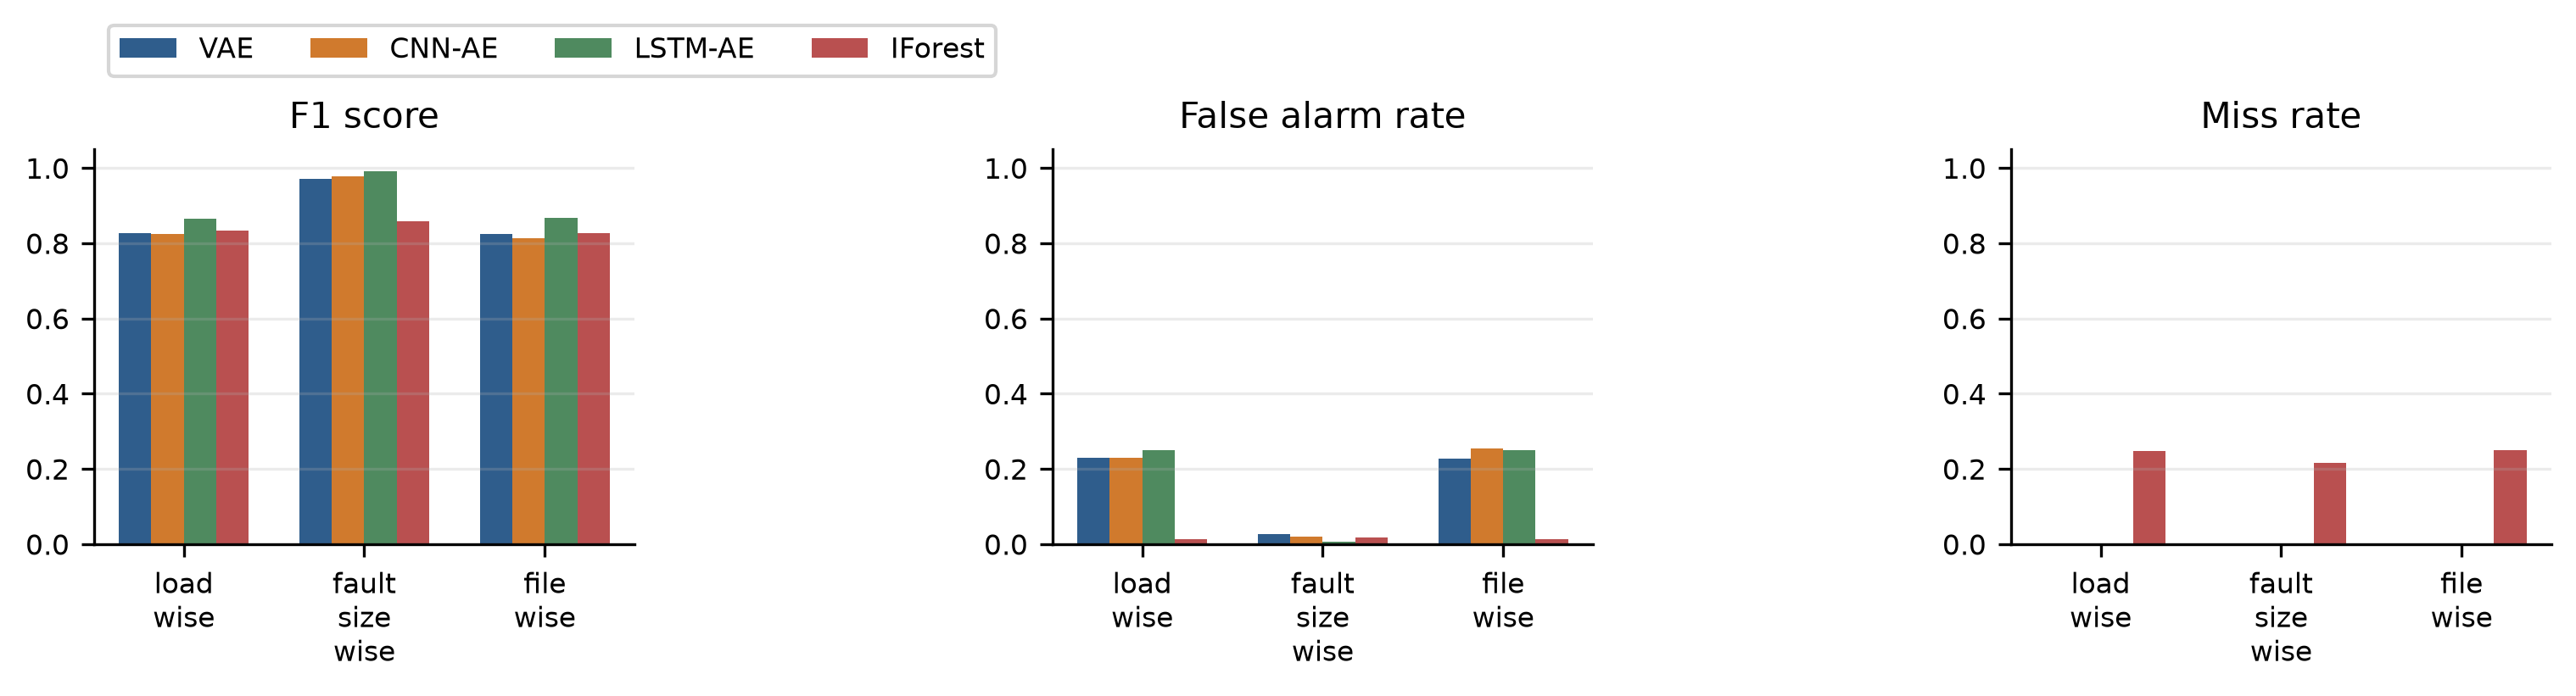
\includegraphics[width=\textwidth]{fig02_cwru_strict_models.png}
  \caption{CWRU strict-protocol performance under validation-P99 calibration. High ranking quality does not automatically imply stable false alarm and miss behavior.}
  \label{fig:cwru_models}
\end{figure*}

\begin{table}[t]
\centering
\caption{CWRU results under strict protocols using validation-P99 calibration.}
\label{tab:cwru_strict}
\small
\begin{tabular}{llrrrrr}
\toprule
Protocol & Model & ROC-AUC & PR-AUC & F1 & FAR & Miss \\
\midrule
fault-size-wise & CNN-AE & 1.000 & 1.000 & 0.977 & 0.020 & 0.000 \\
fault-size-wise & IForest & 0.984 & 0.966 & 0.858 & 0.017 & 0.216 \\
fault-size-wise & LSTM-AE & 1.000 & 1.000 & 0.992 & 0.007 & 0.000 \\
fault-size-wise & VAE & 1.000 & 1.000 & 0.970 & 0.026 & 0.000 \\
file-wise & CNN-AE & 1.000 & 1.000 & 0.813 & 0.254 & 0.000 \\
file-wise & IForest & 0.977 & 0.940 & 0.827 & 0.014 & 0.250 \\
file-wise & LSTM-AE & 0.997 & 0.981 & 0.868 & 0.250 & 0.000 \\
file-wise & VAE & 1.000 & 1.000 & 0.824 & 0.228 & 0.000 \\
load-wise & CNN-AE & 1.000 & 1.000 & 0.825 & 0.229 & 0.000 \\
load-wise & IForest & 0.978 & 0.941 & 0.833 & 0.014 & 0.247 \\
load-wise & LSTM-AE & 0.999 & 0.989 & 0.866 & 0.250 & 0.000 \\
load-wise & VAE & 1.000 & 1.000 & 0.827 & 0.229 & 0.000 \\
\bottomrule
\end{tabular}
\end{table}

This result changes how the original CWRU finding should be interpreted. A perfect or near-perfect \rocauc\ is not false, but it is incomplete. The more practically relevant observation is that calibration determines whether the model becomes sensitive, conservative or alarm-heavy under a held-out load or file.

\subsection{Paderborn window-length sensitivity}

The Paderborn dataset creates a different picture. Figure~\ref{fig:paderborn_window} shows that the selected window length affects F1 under condition-wise protocols. Shorter windows can be insufficient because they capture less rotational and fault-pattern context. The main Paderborn experiments therefore use $L=8192$, while 1024, 2048 and 4096 are treated as sensitivity settings.

\begin{figure}[t]
  \centering
  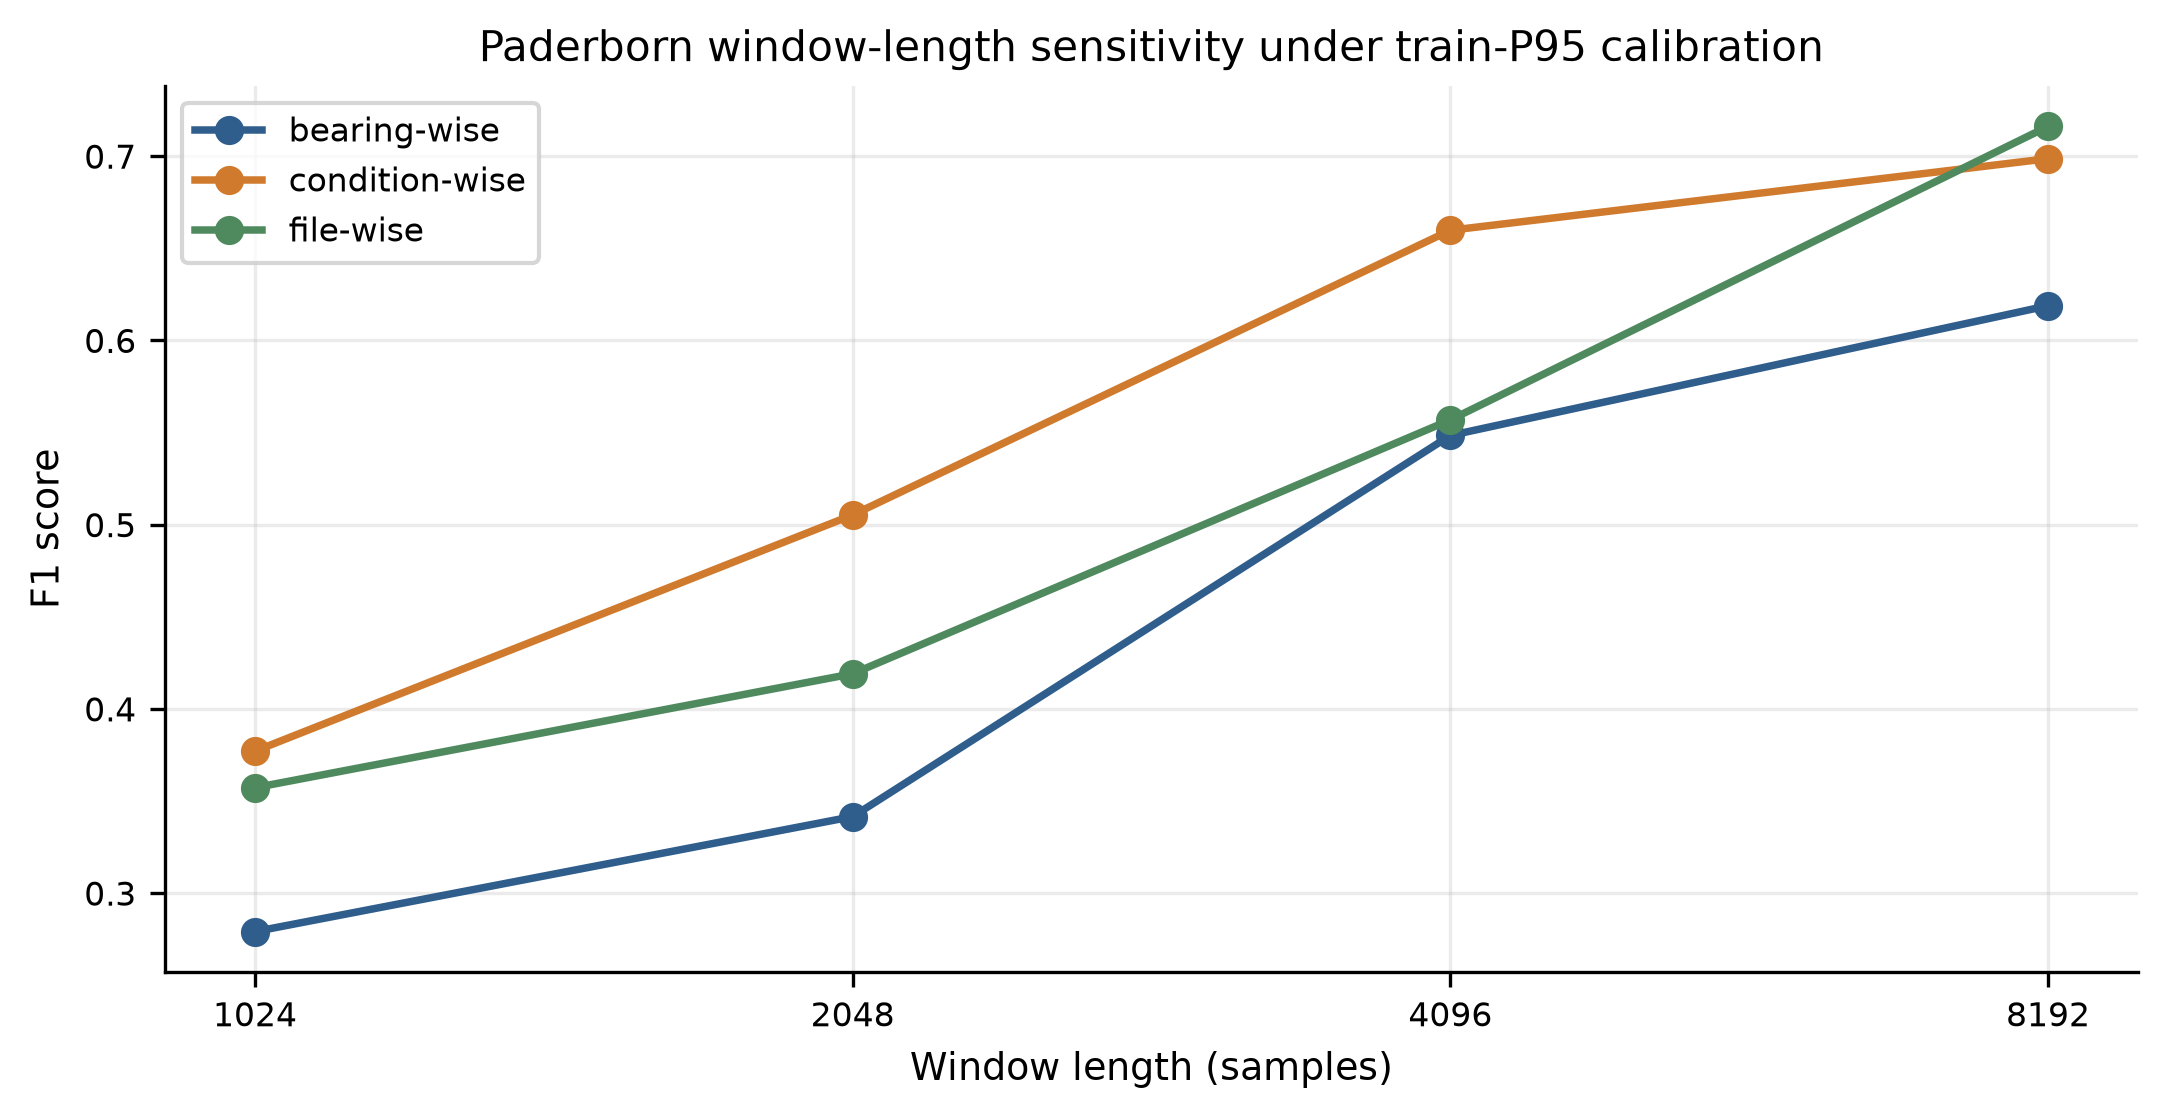
\includegraphics[width=0.95\linewidth]{fig03_paderborn_window_sensitivity.png}
  \caption{Paderborn window-length sensitivity under train-P95 calibration. The external dataset requires longer context than the original CWRU-centered setting.}
  \label{fig:paderborn_window}
\end{figure}

The important point is not that 8192 is universally optimal. Rather, Paderborn demonstrates that preprocessing choices tuned on CWRU do not automatically transfer to external datasets. This supports the decision to include dataset-specific sensitivity analysis in a journal version.

\subsection{External Paderborn validation}

Figure~\ref{fig:paderborn_heatmap} and Table~\ref{tab:paderborn_external} summarize Paderborn results under validation-P95 calibration. Unlike CWRU, Paderborn does not produce uniformly high thresholded performance. The heatmap shows that ranking quality and F1 can diverge across protocols and models. In particular, external bearing and condition variation makes fault detection substantially harder for reconstruction models, while Isolation Forest remains competitive in several thresholded settings.

\begin{figure*}[t]
  \centering
  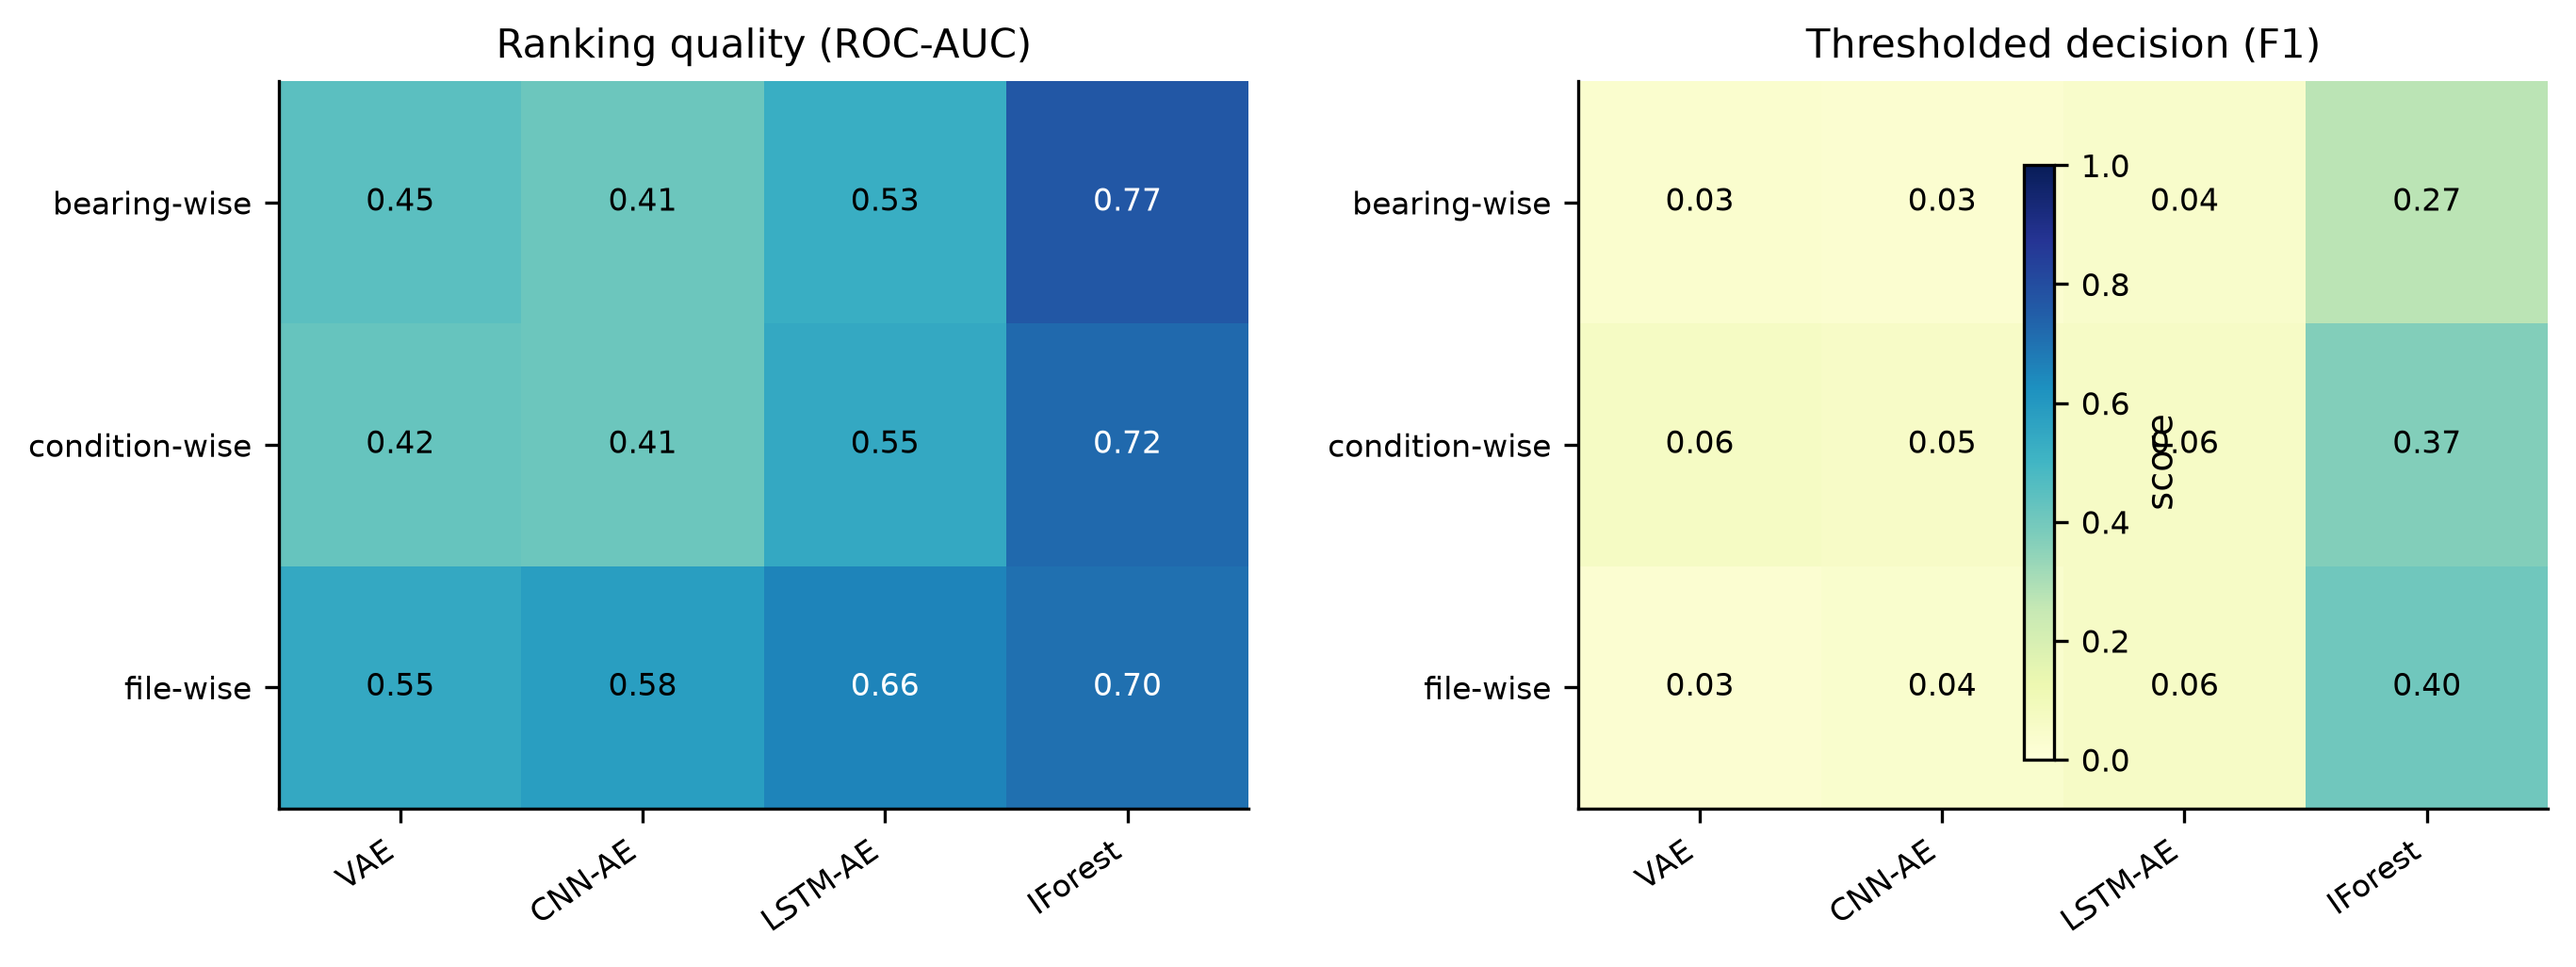
\includegraphics[width=0.95\textwidth]{fig04_paderborn_protocol_heatmap.png}
  \caption{Paderborn external validation under validation-P95 calibration. The heatmap separates ranking quality from thresholded decision quality.}
  \label{fig:paderborn_heatmap}
\end{figure*}

\begin{table}[t]
\centering
\caption{Paderborn external validation results under validation-P95 calibration.}
\label{tab:paderborn_external}
\small
\begin{tabular}{llrrrrr}
\toprule
Protocol & Model & ROC-AUC & PR-AUC & F1 & FAR & Miss \\
\midrule
bearing-wise & CNN-AE & 0.411 & 0.627 & 0.028 & 0.058 & 0.986 \\
bearing-wise & IForest & 0.767 & 0.847 & 0.273 & 0.051 & 0.827 \\
bearing-wise & LSTM-AE & 0.525 & 0.687 & 0.044 & 0.046 & 0.977 \\
bearing-wise & VAE & 0.447 & 0.646 & 0.033 & 0.058 & 0.982 \\
condition-wise & CNN-AE & 0.413 & 0.416 & 0.055 & 0.108 & 0.959 \\
condition-wise & IForest & 0.720 & 0.737 & 0.368 & 0.146 & 0.735 \\
condition-wise & LSTM-AE & 0.547 & 0.500 & 0.060 & 0.052 & 0.967 \\
condition-wise & VAE & 0.424 & 0.421 & 0.063 & 0.122 & 0.949 \\
file-wise & CNN-AE & 0.579 & 0.839 & 0.037 & 0.033 & 0.981 \\
file-wise & IForest & 0.704 & 0.883 & 0.403 & 0.140 & 0.718 \\
file-wise & LSTM-AE & 0.656 & 0.863 & 0.062 & 0.034 & 0.968 \\
file-wise & VAE & 0.547 & 0.826 & 0.026 & 0.027 & 0.987 \\
\bottomrule
\end{tabular}
\end{table}

These results are less visually impressive than CWRU, but they are scientifically more informative. They reveal the point at which a clean benchmark workflow encounters realistic domain variation. For a journal article, this is a strength rather than a weakness because it prevents the study from claiming unrealistic generalization.

\subsection{Threshold calibration behavior}

Threshold calibration is the core experimental contribution of the journal version. Figure~\ref{fig:dataset_calibration} compares dataset-level calibration policies. On CWRU, percentile policies remain strong and robust MAD behaves conservatively. On Paderborn, however, P99 and MAD thresholds become too conservative and miss most faults. Train-P95 and validation-P95 provide more practical operating points, but still show higher miss rates than CWRU.

\begin{figure*}[t]
  \centering
  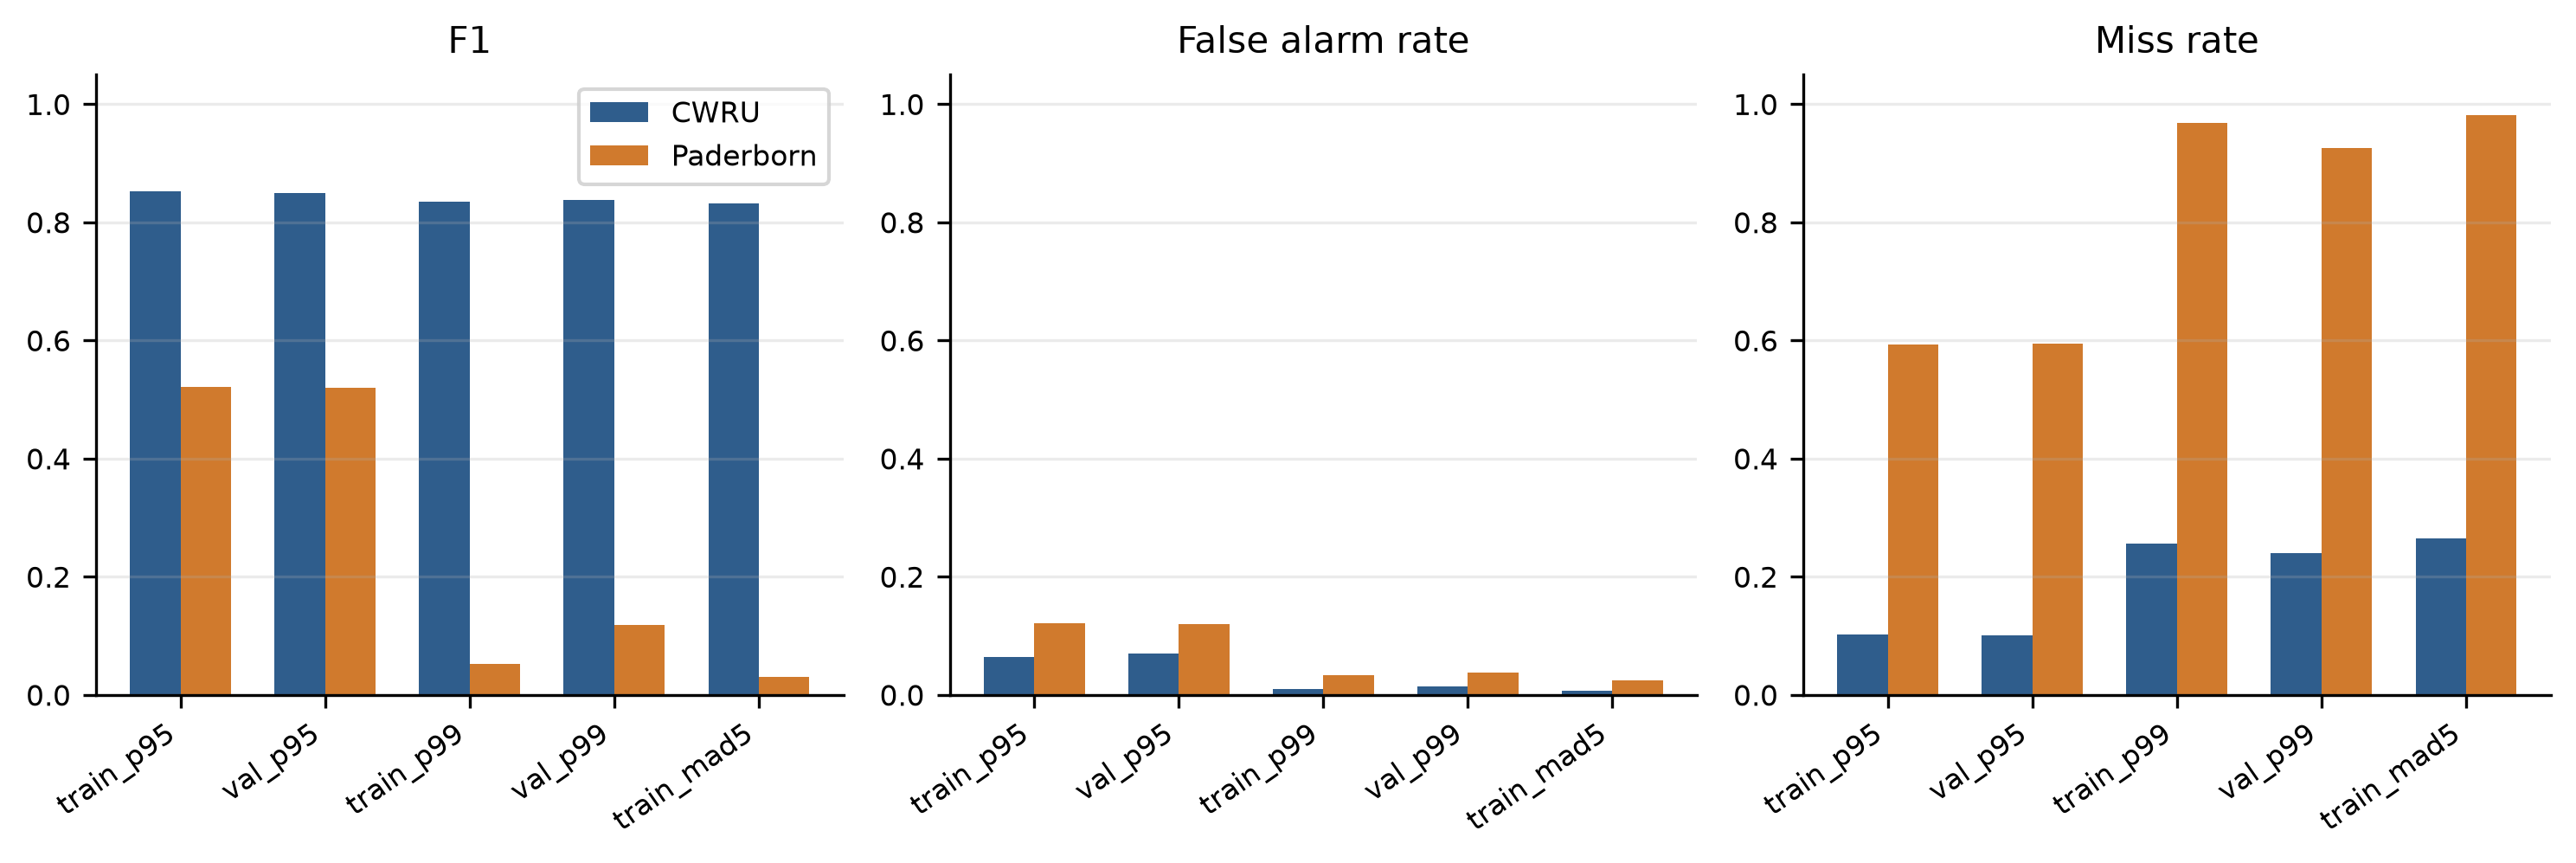
\includegraphics[width=\textwidth]{fig05_dataset_calibration_tradeoff.png}
  \caption{Dataset-level threshold calibration comparison. CWRU and Paderborn have similar score-pipeline structure but very different threshold transfer behavior.}
  \label{fig:dataset_calibration}
\end{figure*}

\begin{table}[t]
\centering
\caption{Dataset-level threshold calibration comparison for the Isolation Forest score.}
\label{tab:calibration_policies}
\small
\begin{tabular}{llrrrrr}
\toprule
Dataset & Policy & ROC-AUC & PR-AUC & F1 & FAR & Miss \\
\midrule
CWRU & train\_mad5 & 0.979 & 0.948 & 0.832 & 0.008 & 0.264 \\
CWRU & train\_p95 & 0.979 & 0.948 & 0.852 & 0.065 & 0.102 \\
CWRU & train\_p99 & 0.979 & 0.948 & 0.834 & 0.010 & 0.256 \\
CWRU & val\_p95 & 0.979 & 0.948 & 0.849 & 0.070 & 0.101 \\
CWRU & val\_p99 & 0.979 & 0.948 & 0.838 & 0.015 & 0.240 \\
Paderborn & train\_mad5 & 0.785 & 0.836 & 0.030 & 0.024 & 0.981 \\
Paderborn & train\_p95 & 0.785 & 0.836 & 0.522 & 0.122 & 0.594 \\
Paderborn & train\_p99 & 0.785 & 0.836 & 0.053 & 0.033 & 0.969 \\
Paderborn & val\_p95 & 0.785 & 0.836 & 0.520 & 0.119 & 0.595 \\
Paderborn & val\_p99 & 0.785 & 0.836 & 0.118 & 0.038 & 0.926 \\
\bottomrule
\end{tabular}
\end{table}

Figure~\ref{fig:paderborn_threshold_rates} further shows how Paderborn thresholds trade false alarms against missed detections across protocols. This figure is especially important for industrial health monitoring. It demonstrates that a threshold cannot be chosen only because it looks statistically conservative on normal training scores. If the threshold is too conservative, the alarm system becomes quiet but misses faults.

\begin{figure}[t]
  \centering
  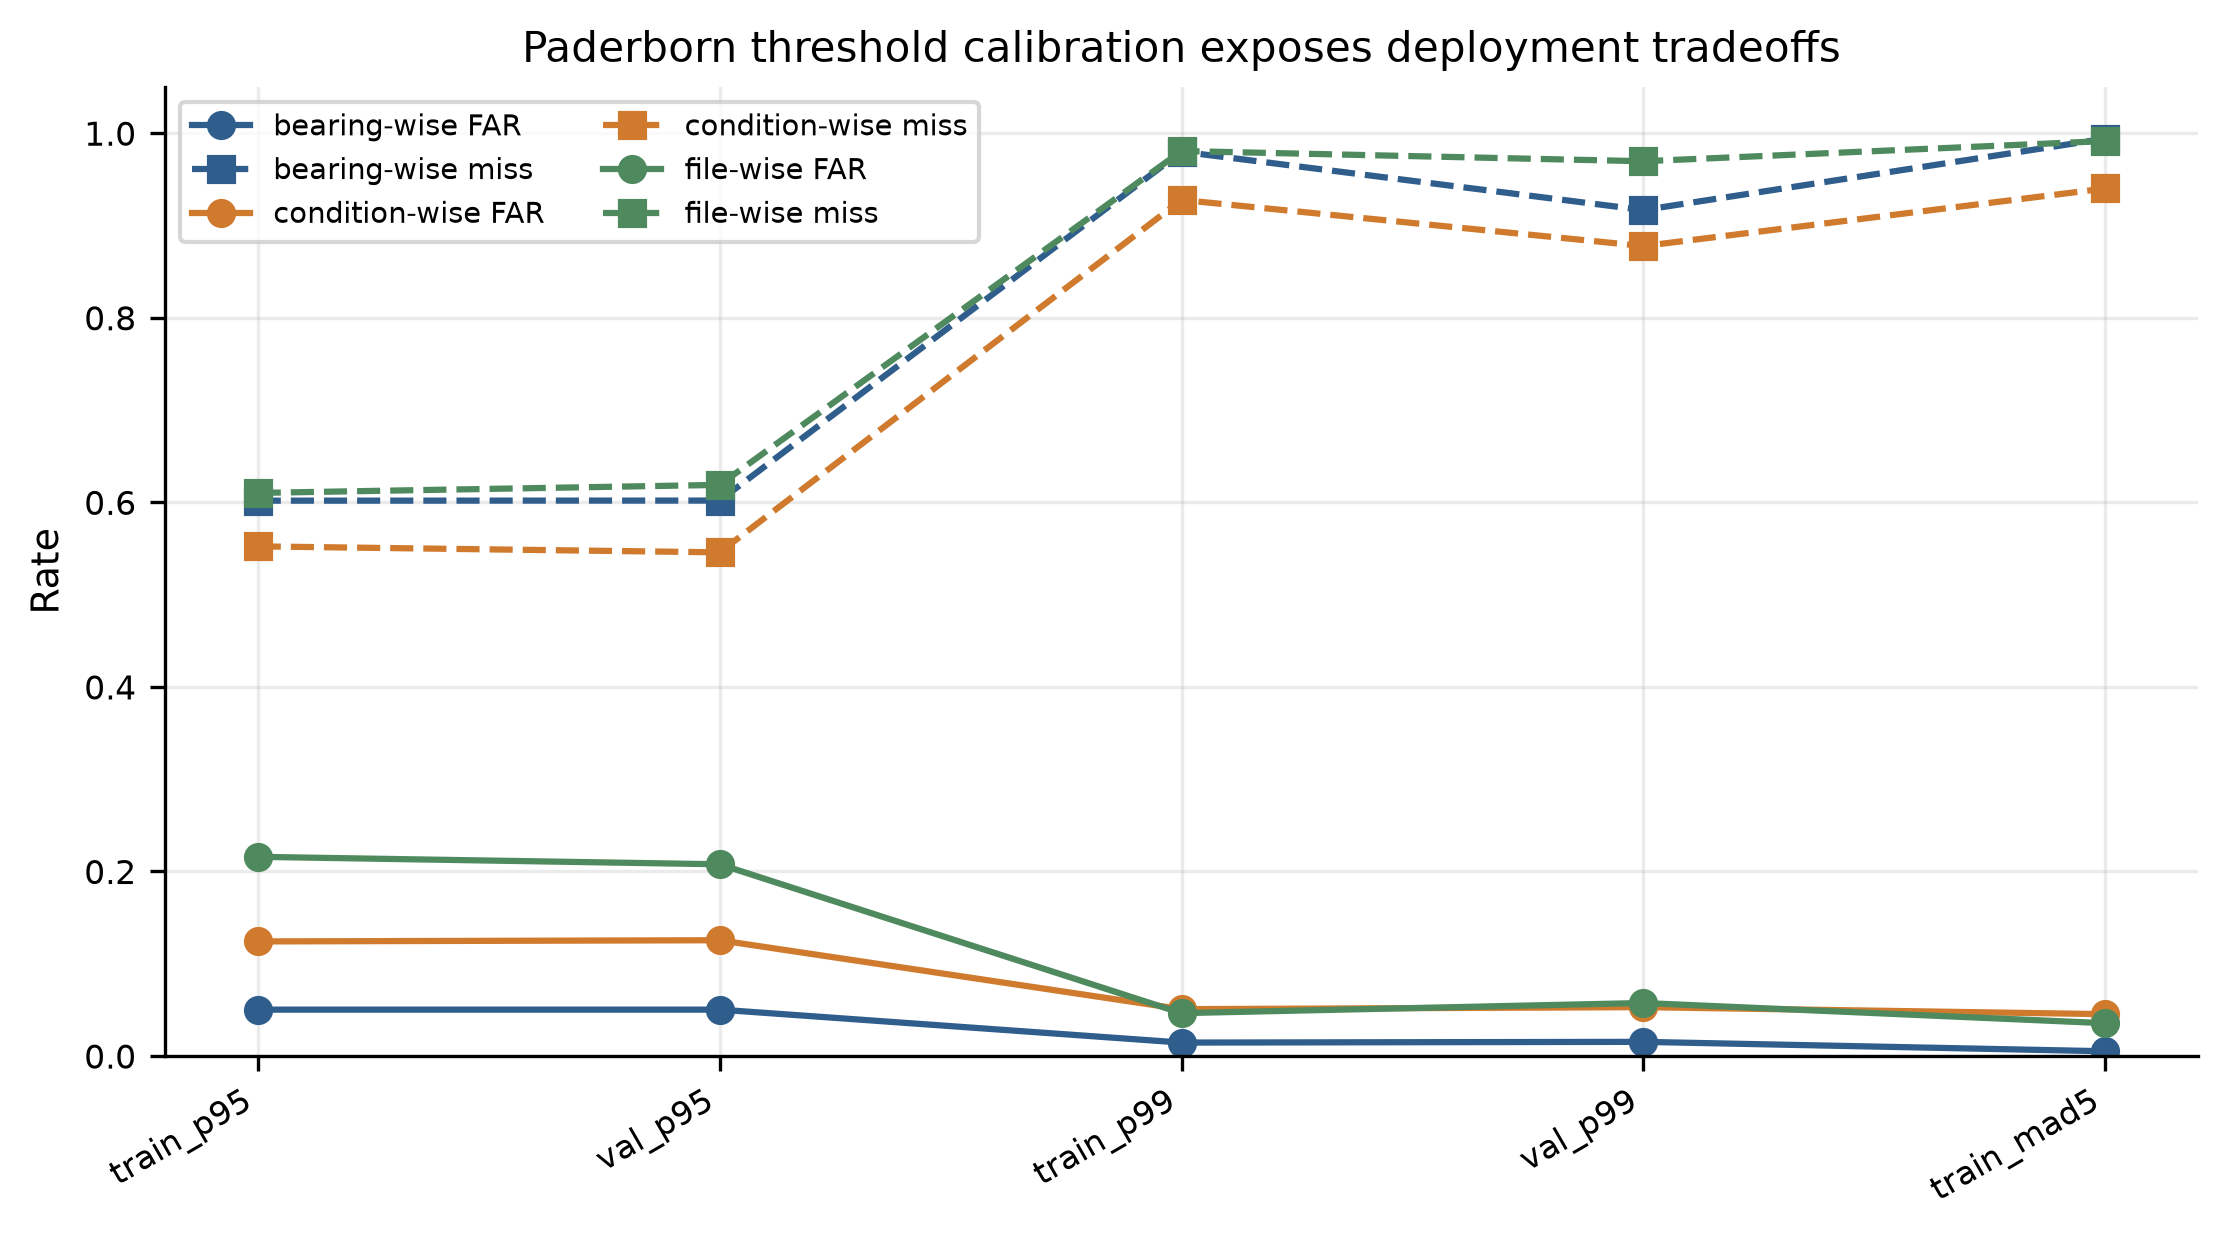
\includegraphics[width=0.98\linewidth]{fig06_paderborn_threshold_rates.png}
  \caption{Paderborn threshold calibration exposes deployment tradeoffs. Conservative thresholds reduce false alarms but can miss most abnormal windows.}
  \label{fig:paderborn_threshold_rates}
\end{figure}

This supports a key recommendation: future bearing anomaly detection studies should report threshold sensitivity as a primary result, not as an optional appendix.

\subsection{Fuzzy health index}

The fuzzy layer converts calibrated scores into a health index and decision regions. Figure~\ref{fig:fuzzy_policy} compares hard P95, warning-as-alarm and fault-only fuzzy policies. On CWRU, fault-only fuzzy decision reduces false alarms while maintaining useful F1. On Paderborn, the same policy becomes too conservative because many fault windows fall into lower-confidence regions. Warning-as-alarm recovers sensitivity but increases false alarms.

\begin{figure}[t]
  \centering
  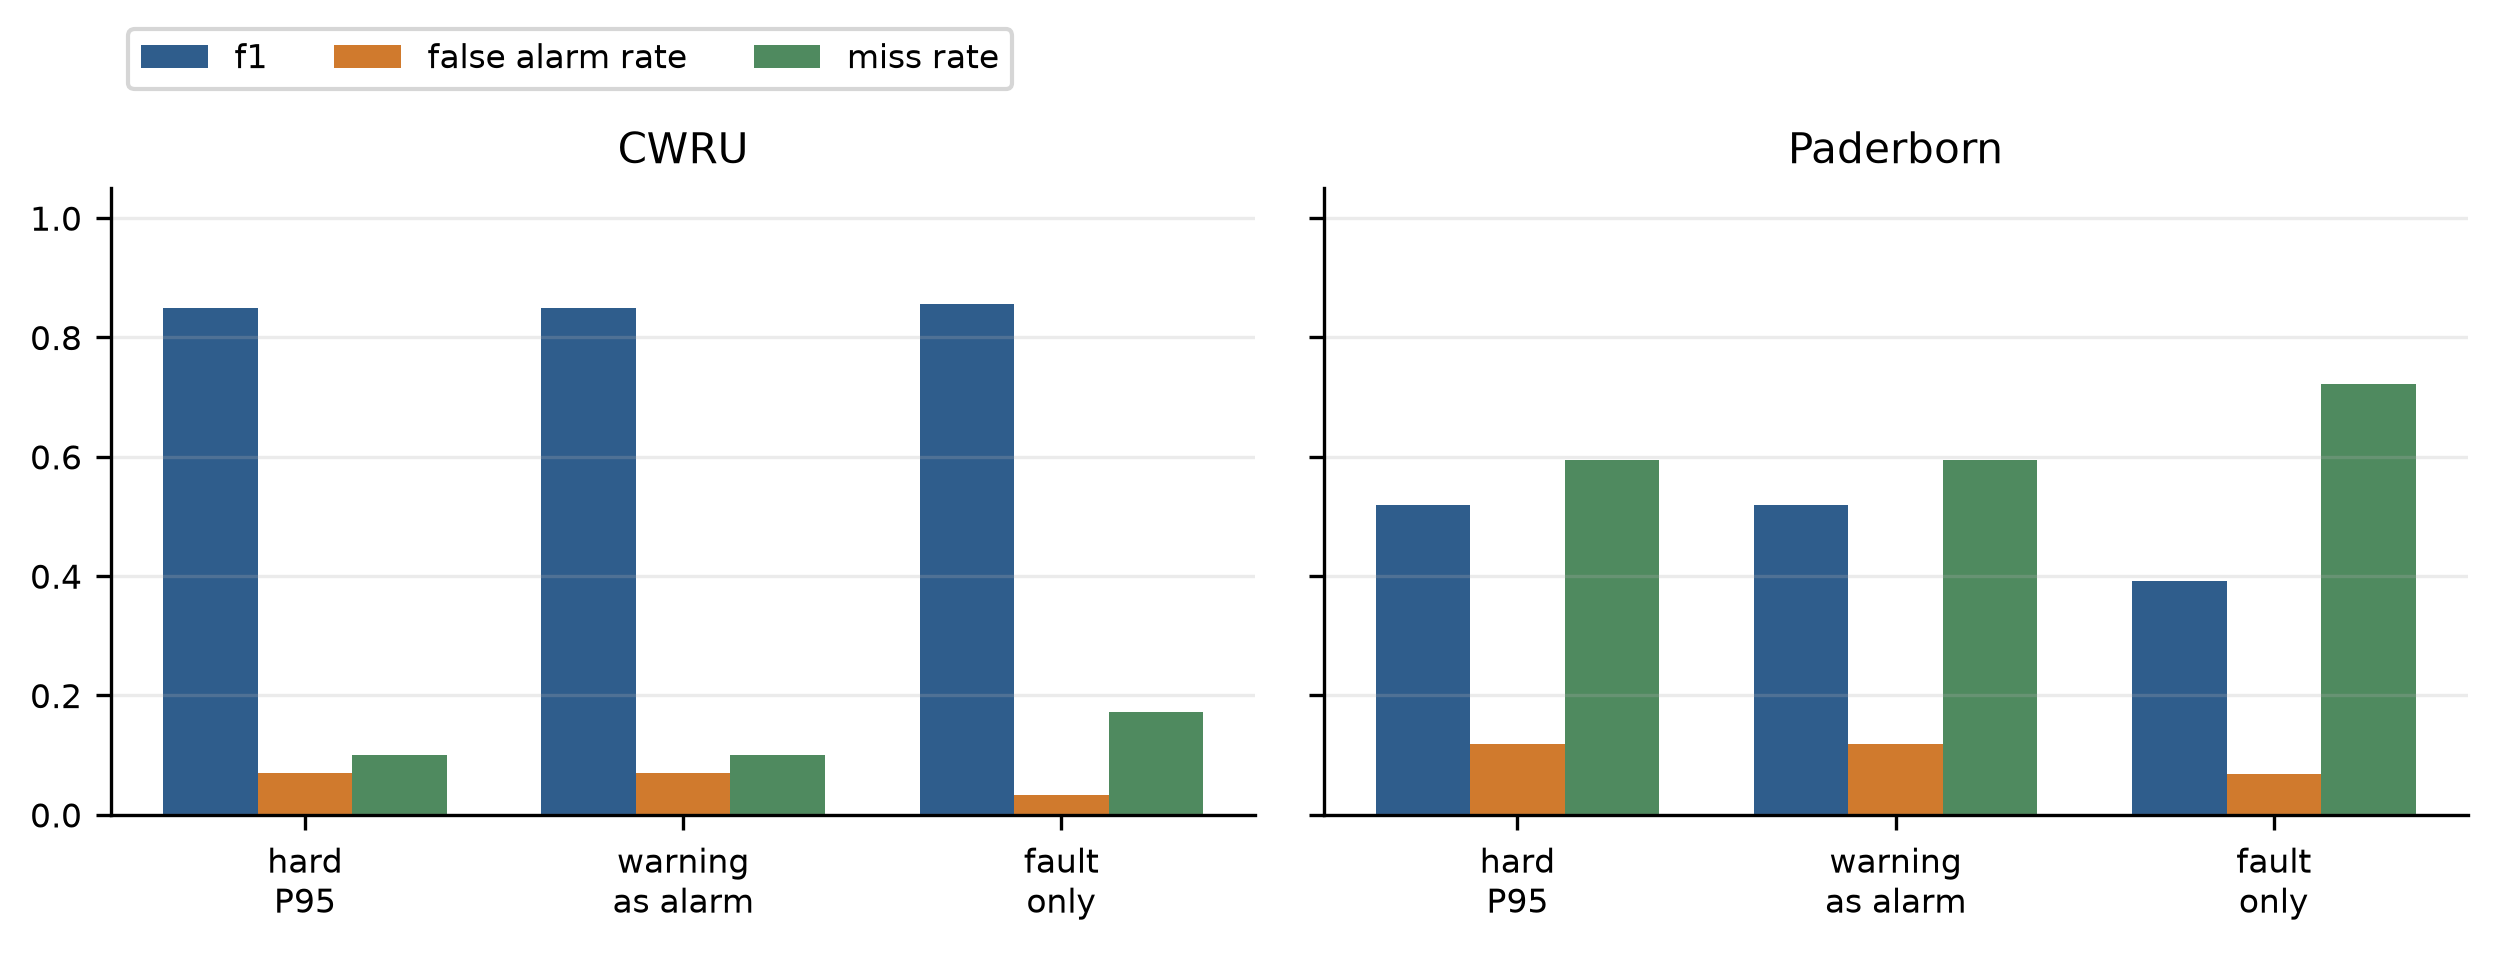
\includegraphics[width=0.98\linewidth]{fig07_fuzzy_policy_comparison.png}
  \caption{Fuzzy policy comparison. Warning-as-alarm and fault-only policies encode different operating risk preferences.}
  \label{fig:fuzzy_policy}
\end{figure}

Table~\ref{tab:fuzzy_health} reports the same behavior numerically. The value of the fuzzy layer is not that it magically improves all metrics. Its value is that it makes the tradeoff explicit and offers a graded health signal for operator-facing monitoring.

\begin{table}[t]
\centering
\caption{Fuzzy health decision policies and health-index separation.}
\label{tab:fuzzy_health}
\small
\begin{tabular}{llrrrrrr}
\toprule
Dataset & Policy & F1 & FAR & Miss & Uncertain & HI normal & HI fault \\
\midrule
CWRU & fuzzy fault only hi75 & 0.856 & 0.033 & 0.172 & 0.087 & 0.112 & 0.888 \\
CWRU & fuzzy warning as alarm hi50 & 0.849 & 0.070 & 0.100 & 0.087 & 0.112 & 0.888 \\
CWRU & hard val p95 & 0.849 & 0.070 & 0.100 & 0.087 & 0.112 & 0.888 \\
Paderborn & fuzzy fault only hi75 & 0.391 & 0.068 & 0.721 & 0.156 & 0.147 & 0.411 \\
Paderborn & fuzzy warning as alarm hi50 & 0.520 & 0.119 & 0.595 & 0.156 & 0.147 & 0.411 \\
Paderborn & hard val p95 & 0.520 & 0.119 & 0.595 & 0.156 & 0.147 & 0.411 \\
\bottomrule
\end{tabular}
\end{table}

Figure~\ref{fig:health_separation} shows mean health-index separation. CWRU produces strong separation between normal and fault windows. Paderborn produces weaker separation and a higher uncertain rate. This pattern matches the earlier threshold results and gives a more interpretable explanation: Paderborn is not merely a lower-scoring dataset; it contains more ambiguous operating regions for a normal-only detector.

\begin{figure*}[t]
  \centering
  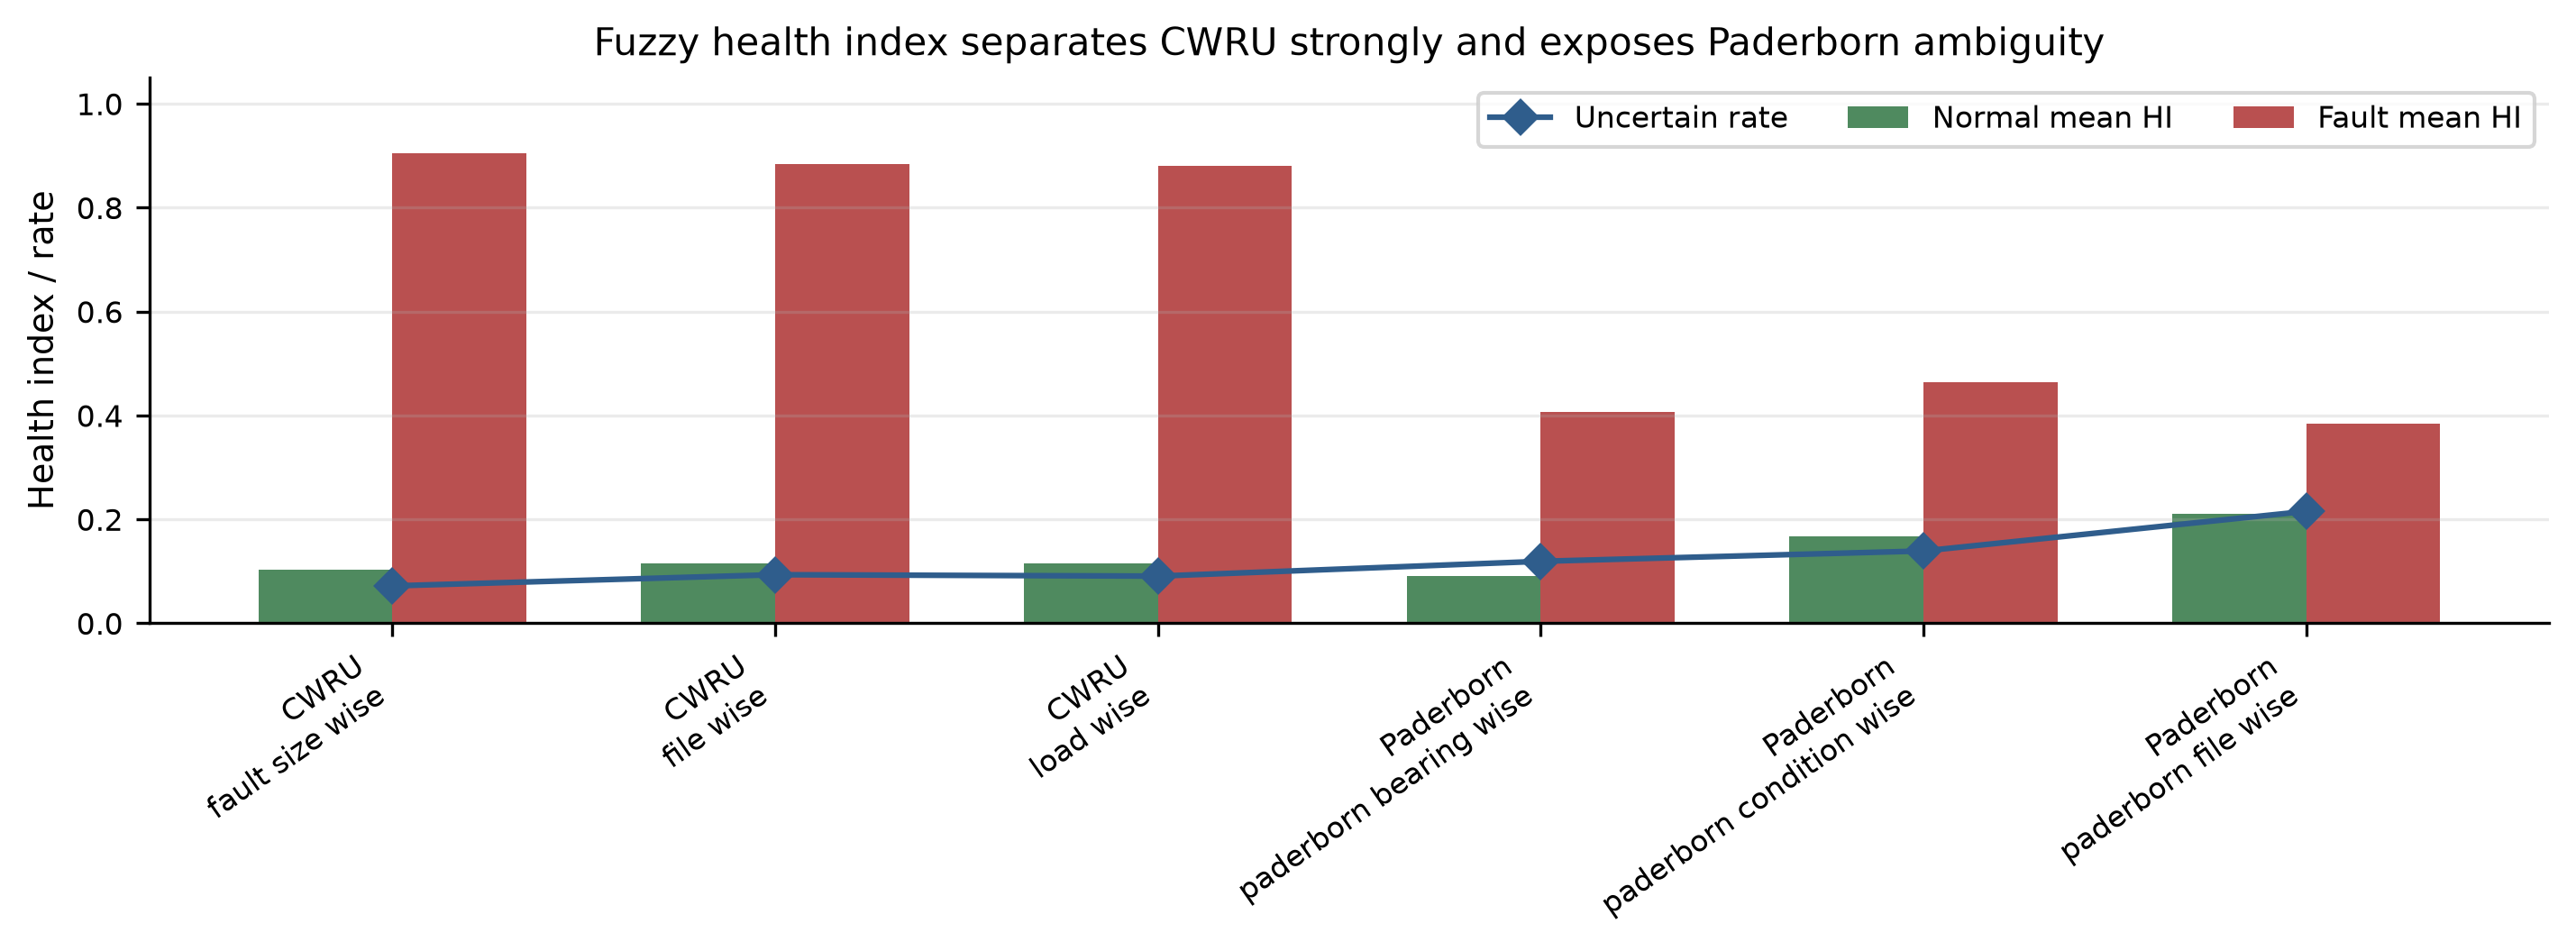
\includegraphics[width=0.95\textwidth]{fig08_health_index_separation.png}
  \caption{Fuzzy health-index separation. CWRU shows strong normal-fault separation, while Paderborn exposes ambiguity that should be reported rather than hidden.}
  \label{fig:health_separation}
\end{figure*}

\subsection{Efficiency and deployability}

Finally, Figure~\ref{fig:efficiency} and Table~\ref{tab:efficiency} summarize computational footprint. LSTM-AE is compact and fast in the current implementation. VAE and CNN-AE are larger but remain within a lightweight range for offline or near-real-time window-level monitoring. Isolation Forest has negligible neural model size and inference overhead, making it attractive as a baseline or embedded screening method.

\begin{figure}[t]
  \centering
  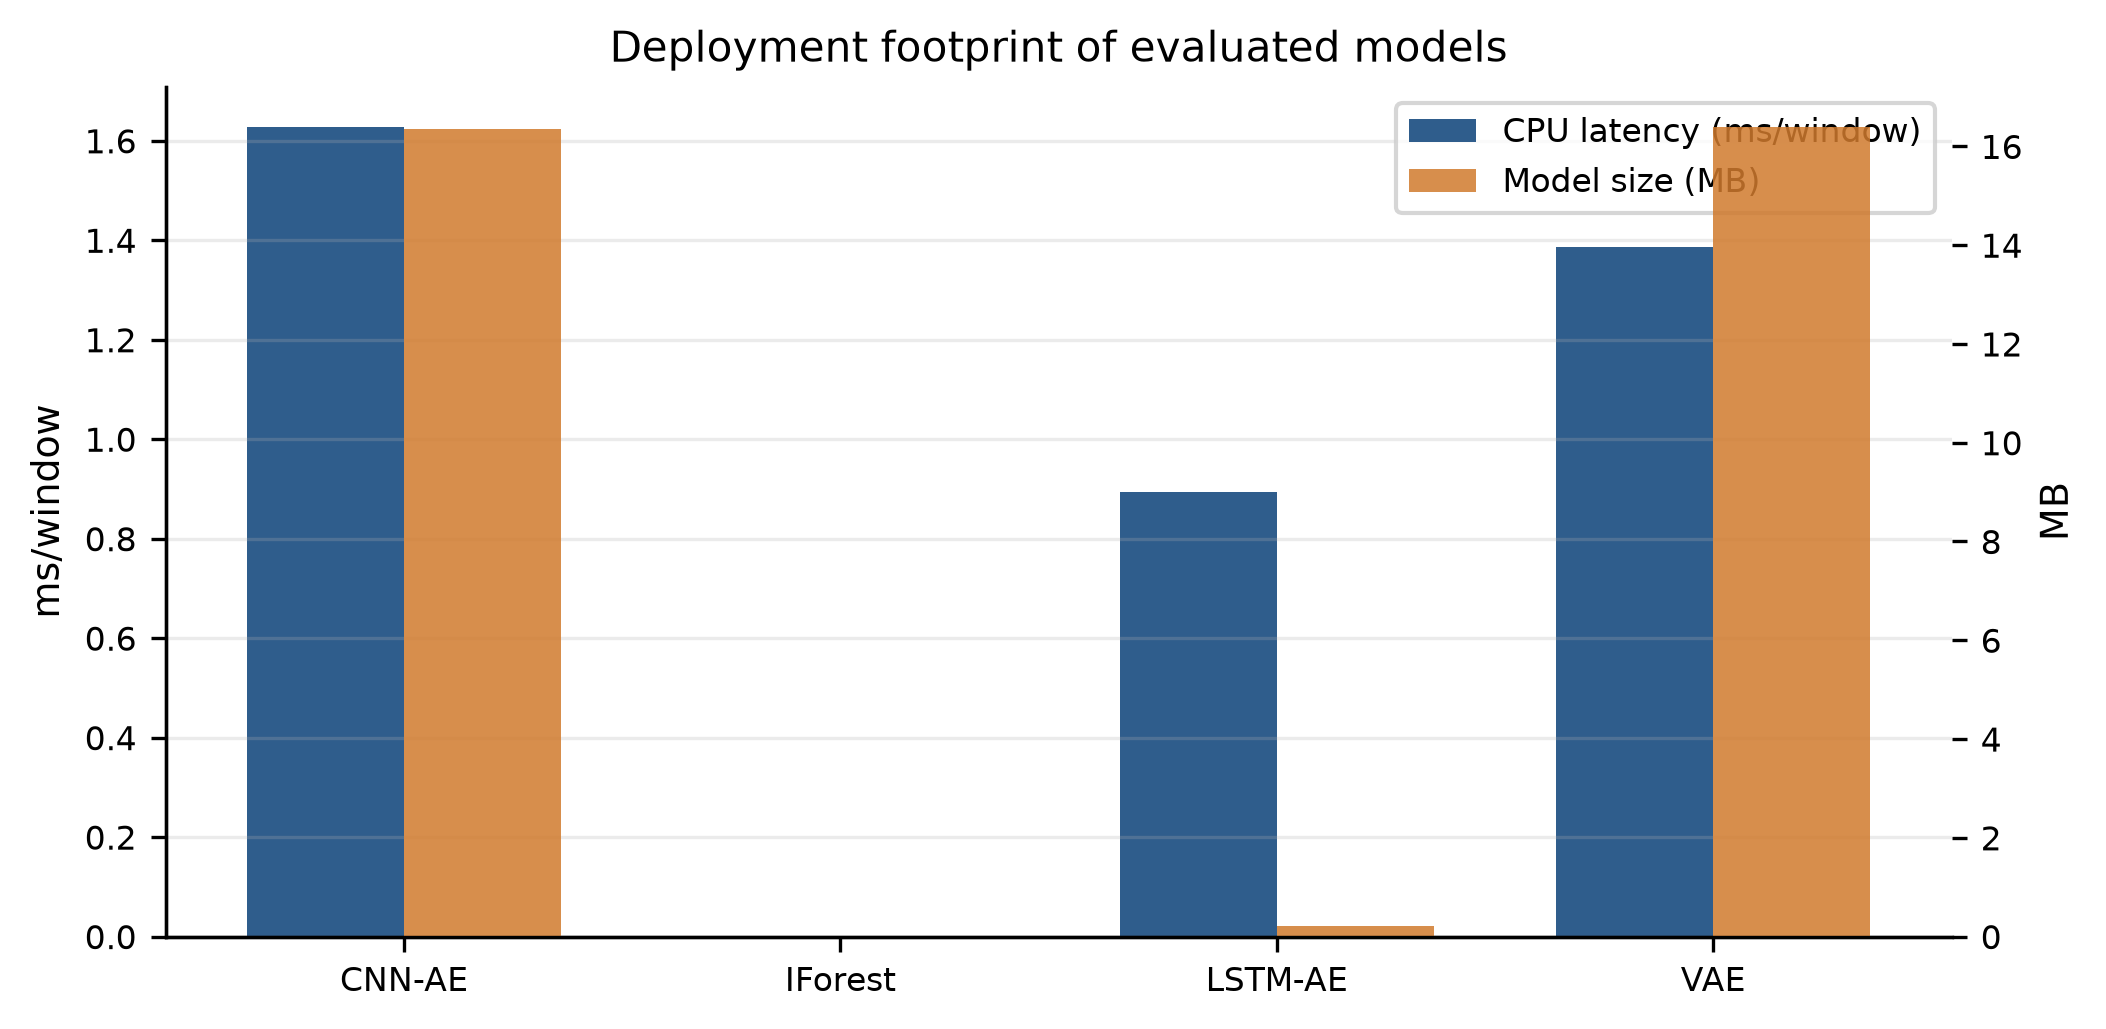
\includegraphics[width=0.95\linewidth]{fig09_efficiency_footprint.png}
  \caption{Deployment footprint of evaluated models. CPU latency and model size should be reported together with accuracy metrics.}
  \label{fig:efficiency}
\end{figure}

\begin{table}[t]
\centering
\caption{CPU inference latency and model footprint measured per window.}
\label{tab:efficiency}
\small
\begin{tabular}{lrrr}
\toprule
Model & CPU ms/window & Size MB & Parameters \\
\midrule
CNN-AE & 1.627 & 16.357 & 4287265 \\
IForest & 0.000 & 0.000 & 300 \\
LSTM-AE & 0.893 & 0.209 & 54689 \\
VAE & 1.385 & 16.389 & 4295489 \\
\bottomrule
\end{tabular}
\end{table}

The efficiency results do not by themselves prove field deployment readiness. They do, however, provide evidence that the workflow is computationally plausible and that future deployment studies can focus on streaming integration, sensor hardware and plant-specific calibration.

\section{Discussion}
\label{sec:discussion}

The results support a more careful interpretation of bearing anomaly detection research. If the study only reported CWRU \rocauc, it would be tempting to claim that reconstruction models solve the problem. Once strict splits, Paderborn validation and threshold policies are included, the conclusion becomes more useful: ranking can remain strong while calibration and health decisions remain fragile.

\subsection{Why imperfect Paderborn results are valuable}

The Paderborn results are not a failure of the study. They are evidence that external validation is necessary. A journal paper should not hide the fact that performance drops when moving from CWRU to broader bearing data. Instead, the drop should be analyzed because it reveals what must be solved before deployment: cross-condition calibration, bearing-specific score shifts and threshold sensitivity.

This is also where the paper's contribution differs from a conventional model-comparison study. The objective is not to select one universal winner among VAE, CNN-AE, LSTM-AE and Isolation Forest. The objective is to show how each model behaves when the same calibration and health-decision framework is applied. Under this view, a simpler model with clearer calibration behavior may be more useful than a complex model with excellent ranking but unstable alarm rates.

\subsection{Threshold calibration as a core contribution}

The experiments show that threshold calibration should be treated as a core method component. CWRU and Paderborn have different score distributions, and conservative thresholds do not transfer uniformly. A threshold that is attractive because it produces few false alarms can also produce unacceptable miss rates. This is particularly important for industrial health monitoring because false alarms and missed faults carry different costs depending on the plant.

The proposed workflow does not prescribe one threshold for all cases. Instead, it makes threshold choice auditable. Train-P95, validation-P95, P99 and MAD policies can be compared under the same metrics, allowing users to select operating points according to risk preference. This is more honest than reporting a single optimized threshold without explaining how it was obtained.

\subsection{Role of the fuzzy health index}

The fuzzy health index complements threshold calibration. In a clean benchmark, the fuzzy output mostly confirms strong separation. In Paderborn, it reveals uncertain regions and weaker health-index separation. This makes the fuzzy layer useful as an interpretability mechanism even when it does not improve F1. For operators, a warning or uncertain state is more informative than a silent binary classifier that hides score ambiguity.

The fuzzy layer is also model-agnostic. Although the current figures emphasize Isolation Forest and reconstruction-score settings, the same mapping can be applied to VAE, CNN-AE and LSTM-AE scores after normalization. This means the health-decision component can remain stable even if the anomaly model is replaced.

\subsection{Limitations}

Several limitations remain. First, the study uses public datasets rather than private plant data. Public datasets are necessary for reproducibility, but they cannot fully capture sensor aging, installation variation, maintenance logs or operator interventions. Second, the Paderborn experiments improve external validation but do not exhaust all possible fault modes or operating regimes. Third, the fuzzy membership functions are calibrated from score anchors rather than optimized from plant-specific cost functions. Fourth, the present paper does not include federated learning. Privacy-preserving multi-plant learning is an important future direction, but including it here would dilute the main contribution and require a separate experimental design.

\subsection{Implications for journal submission}

For journal submission, the strongest positioning is not model novelty. The strongest positioning is evaluation maturity. The paper provides a reproducible workflow that converts a clean CWRU-centered conference study into a more rigorous journal study by adding strict splits, external Paderborn validation, threshold calibration, fuzzy health interpretation and deployment metrics. This is a credible contribution for journals interested in applied artificial intelligence, mechanical condition monitoring and intelligent maintenance, provided that the manuscript is framed as a workflow and evaluation study rather than a state-of-the-art architecture paper.

\section{Conclusion}
\label{sec:conclusion}

This paper presented a calibration-aware fuzzy health-index workflow for normal-only bearing anomaly detection. The study began from a VAE-based CWRU anomaly detection pipeline but expanded the evaluation to include strict CWRU protocols, an external Paderborn dataset, multiple baselines, threshold calibration policies and fuzzy health-state decisions. The results show that CWRU can remain highly separable under stricter splits, but thresholded behavior still depends on calibration. Paderborn external validation is substantially harder and exposes the practical importance of false alarm, miss rate and uncertainty reporting. The fuzzy health index provides an interpretable decision layer that makes warning and ambiguous regions visible.

The main lesson is that deployable bearing anomaly detection cannot be judged by \rocauc\ alone. A useful study should report how scores are calibrated, how thresholds transfer, how decisions behave under external conditions and how the system can be reproduced. Future work will extend the workflow to privacy-preserving federated learning and plant-specific adaptive calibration while keeping normal-only training as the central industrial assumption.

\section*{Data and Code Availability}

The experimental workflow, generated CSV summaries, figures and LaTeX tables are organized to support reproducible execution. Public datasets should be downloaded from the original CWRU and Paderborn sources according to their respective usage terms.

\section*{Conflict of Interest}

The authors declare no conflict of interest.

\bibliographystyle{unsrtnat}
\bibliography{references}

\end{document}
